\RequirePackage{plautopatch}
\documentclass[uplatex, a4paper, 14Q, dvipdfmx]{jsarticle}
\usepackage{docmute}
\usepackage{../mypackage}

\title{安定\texorpdfstring{$\infty$}{infty}圏}
\author{よの}
\date{\today}

\begin{document}

\maketitle

\begin{abstract}
\end{abstract}

\tableofcontents

\section{安定\texorpdfstring{$\infty$}{infty}圏}

\subsection{安定性}

\begin{definition}[始対象と終対象]
  $\C$を$\infty$圏とする.
  $\C$のある対象$\emptyset$が, 任意の$X \in \C$に対して$\Map_\C(\emptyset,X)$が可縮なKan複体であるとき, $\emptyset$を始対象(initial object)という. 

  双対的に, $\C$のある対象$1$が, 任意の$X \in \C$に対して$\Map_\C(X,1)$が可縮なKan複体であるとき, $1$を終対象(terminal object)という. 
\end{definition}

\begin{definition}[基点付き$\infty$圏]
  $\C$を$\infty$圏とする.
  $\C$のある対象$0$が始対象かつ終対象であるとき, $0$を零対象(zero object)という.
  $\C$が零対象を持つとき, $\C$は基点付き(pointed)であるという.
\end{definition}

\begin{remark}
  零対象は存在すれば同型を除いて一意である. 
\end{remark}

\begin{definition}[ヌルホモトピー]
  $\C$を基点付き$\infty$圏, $f : X \to Y$を$\C$の射とする.
  次の図式で表される$2$単体$\Delta^2 \to \C$を$f$のヌルホモトピーという.
  また, ヌルホモトピーを持つ$f$を$0$射($0$-map)という. 
  \[
    \begin{tikzpicture}[auto,->]
      \node (0) at (1,0) {$0$};
      \node (X) at (0,1) {$X$};
      \node (Y) at (2,1) {$Y$};
      \draw (X) -- node {$f$} (Y);
      \draw (X) -- (0);
      \draw (0) -- (Y);
    \end{tikzpicture}
  \]
\end{definition}

\begin{lemma}
  $\C$を$\infty$圏とする.
  $\C$が基点付きであることと, 次の3つの条件を満たすことは同値である. 
  \begin{enumerate}
    \item $\C$は始対象$\emptyset$を持つ.
    \item $\C$は終対象$1$を持つ. 
    \item $\C$の射$f : 1 \to \emptyset$が存在する. 
  \end{enumerate}
\end{lemma}

\begin{proof}
  $\C$が基点付きであるとき, 3つの条件を満たすことは明らかである. 

  逆に, 条件(1)から(3)が満たされているとする.
  $\emptyset$は始対象なので, 射$g : \emptyset \to 1$が存在する.
  $\emptyset$は始対象なので, $fg \simeq \id_\emptyset$である.
  $1$は終対象なので, $gf \simeq \id_1$である. 
  よって, $g$は$f$のホモトピー逆射なので, $f$は同型射である.
  従って, $\emptyset$は終対象でもあるので, $\C$は基点付きである. 
\end{proof}

\begin{definition}[(コ)ファイバー]
  $\C$を基点付き$\infty$圏とする.
  次の形で表される射$\Delta^1 \times \Delta^1 \to \C$を$\C$の三角(diagram)という. 
  \[
    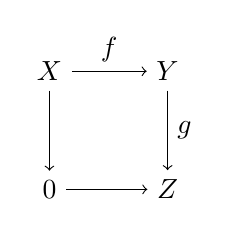
\begin{tikzpicture}[auto,->]
      \node (0) at (0,0) {$0$};
      \node (Z) at (1.5,0) {$Z$};
      \node (X) at (0,1.5) {$X$};
      \node (Y) at (1.5,1.5) {$Y$};
      \draw (0) -- (Z);
      \draw (X) -- (0);
      \draw (X) -- node{$f$} (Y);
      \draw (Y) -- node{$g$} (Z);
    \end{tikzpicture}
  \]
  この三角がpullbackであるとき, 三角をファイバー列(fibre sequence)という.
  双対的に, この三角がpushoutであるとき, 三角をコファイバー列(cofibre sequence)という.

  このようなファイバー列が存在するとき, $g$はファイバーを持つという. 
  双対的に, このようなコファイバー列が存在するとき, $f$はコファイバーを持つという. 
  このとき, $X:=\fib(g), Z := \cofib(f)$と表す. 

  また, $\C$の任意の射が(コ)ファイバーを持つとき, $\C$は(コ)ファイバーを持つという. 
\end{definition}

\begin{remark}
  $\C$を基点付き$\infty$圏とする.
  $\C$の三角は次のデータから構成される.
  \begin{enumerate}
    \item $\C$の射$f : X \to Y$と$g : Y \to Z$
    \item $h$が$g$と$f$の合成であることを表す$2$単体
    \[
      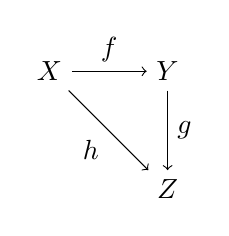
\begin{tikzpicture}[auto,->]
        \node (Z) at (1.5,0) {$Z$};
        \node (X) at (0,1.5) {$X$};
        \node (Y) at (1.5,1.5) {$Y$};
        \draw (X) -- node{$f$} (Y);
        \draw (Y) -- node{$g$} (Z);
        \draw (X) -- node[swap]{$h$} (Z);
      \end{tikzpicture}
    \]
    \item $h$のヌルトピックを表す$2$単体
    \[
      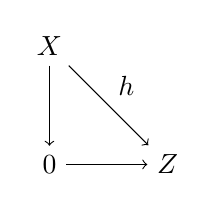
\begin{tikzpicture}[auto,->]
        \node (0) at (0,0) {$0$};
        \node (Z) at (1.5,0) {$Z$};
        \node (X) at (0,1.5) {$X$};
        \draw (0) -- (Z);
        \draw (X) -- (0);
        \draw (X) -- node{$h$} (Z);
      \end{tikzpicture}
    \]
  \end{enumerate} 
\end{remark}

\begin{notation}
  $\C$を基点付き$\infty$圏とする.
  $\C$の三角を次のように表す. 
  \begin{align*}
    X \xrightarrow{f} Y \xrightarrow{g} Z
  \end{align*}
  
\end{notation}

ファイバーやコファイバーをとる操作は関手とみなせる

\begin{remark}
  
\end{remark}

\begin{lemma} \label{prop:cofib_is_left_adj_to_left_Kan_ext}
  
\end{lemma}

\begin{definition}[安定$\infty$圏]
  $\infty$圏$\C$が次の条件を満たすとき, $\C$は安定(stable)であるという. 
  \begin{description}
    \item[(S1)] $\C$は基点付きである, つまり零対象$0$を持つ. 
    \item[(S2)] $\C$はファイバーとコファイバーを持つ.
    \item[(S3)] $\C$の三角がファイバー列であることとコファイバー列であることは同値である.
  \end{description}
\end{definition}

\begin{remark}
  安定$\infty$圏の条件(1)はAbel圏における零対象の存在, (2)は核と余核の存在, (3)は準同型定理(射の像と余像が同型である)をそれぞれ表している. 
  つまり, 安定$\infty$圏はAbel圏の無限圏verであると考えられる. 
\end{remark}

\begin{remark}
  安定$\infty$圏は$\infty$圏に追加の構造を持たせたものではなく, $\infty$圏の持つ性質を用いて定義されている. 
\end{remark}

\begin{lemma} \label{prop:Cop_is_also_stable}
  $\C$が安定$\infty$圏であるとき, $\C^\myop$も安定$\infty$圏である.
\end{lemma}

\begin{proof}
  安定$\infty$圏の定義が双対的であることから従う. 
\end{proof}


\subsection{安定\texorpdfstring{$\infty$}{infty}圏のホモトピー圏}

$\infty$圏のホモトピー圏が三角圏の構造を持つ条件について考える. 

$\C$を基点付き$\infty$圏, $0$と$0'$を$\C$の零対象とする. 
次のpushoutで表される図式の$\fun(\Delta^1 \times \Delta^1,\C)$の充満部分圏を$\M^\Sigma$と表す. 
\[
  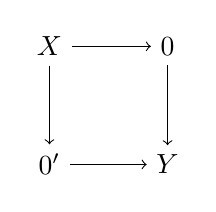
\begin{tikzpicture}[auto,->]
    \node (0') at (0,0) {$0'$};
    \node (Y) at (1.5,0) {$Y$};
    \node (X) at (0,1.5) {$X$};
    \node (0) at (1.5,1.5) {$0$};
    \draw (X) -- (0);
    \draw (X) -- (0');
    \draw (0') -- (Y);
    \draw (0) -- (Y);
  \end{tikzpicture}
\]
HTT.4.3.2.15を2回用いると, 自明なファイブレーション$e : \M^\Sigma \to \C$を得る. 
$s : \C \to \M^\Sigma$を$e$の切断とする.
このとき, 
\begin{align*}
  \Sigma_\C := e \circ s : \C \to \C
\end{align*}
を$\C$上の懸垂(suspention functor)という. 
双対的に, 同じ形のpulbackで表される$\fun(\Delta^1 \times \Delta^1,\C)$の充満部分圏を$\M^\Omega$と表す. 
$\C$がファイバーを持つとき, 同様に自明なファイブレーション$e' : \M^\Omega \to \C$を得る. 
$s' : \C \to \M^\Omega$を$e'$の切断とする.
このとき, 
\begin{align*}
  \Omega\C := e' \circ s' : \C \to \C
\end{align*}
を$\C$上のループ(loop functor)という. 
$\C$が安定であるとき, $\M^\Sigma = \M^\Omega$である. 
よって, 懸垂とループは互いに$\C$上の逆関手である. 

\begin{notation} \label{notation:suspension_and_loop}
  $\C$を安定$\infty$圏とする.
  任意の$X \in \C$と$n \geq 0$に対して, 
  \begin{align*}
    X[n] := \Sigma^n(X)
  \end{align*}
  と表し, 懸垂の$n$乗($n$-th power of the suspension functor)という. 
  $n \leq 0$に対して, 
  \begin{align*}
    X[n] := \Omega^n(X) 
  \end{align*}
  と表し, ループの$-n$乗($(-n)$-th power of the loop functor)という. 
  誘導されるホモトピー圏上の関手の対応も同じ記号を用いて表す.
\end{notation}

\begin{remark}
  $\C$が安定ではない基点付き$\infty$圏のとき, 懸垂とループはホモトピー逆関手ではないが, 随伴ではある.
\end{remark}

\begin{lemma} \label{prop:hc_is_additive}
  $\C$をコファイバーを持つ基点付き$\infty$圏かつ懸垂$\Sigma : \C \to \C$が圏同値であるとする. 
  このとき, $h\C$は加法圏である.
\end{lemma}

\begin{proof}
  $h\C$が有限余直積を持つことを示す. 
  $\C$は終対象を持つので, 2つの対象の余直積を持つことを示せばよい.
  $\cofib : \fun(\Delta^1,\C) \to \C$をコファイバーをとる関手とする. 
  任意の$X,Y \in \C$に対して, 次の同型が存在する. 
  \begin{align*}
    X \cong \cofib(X[-1] \xrightarrow{u} 0), ~~ Y \cong \cofib(0 \xrightarrow{v} Y)
  \end{align*}
  よって, $u \oplus v :X[-1] \to Y$が得られるが, これは$0$射である. 
  \cref{prop:cofib_is_left_adj_to_left_Kan_ext}より, $\cofib$関手は余直積を保つので, 
  \begin{align*}
    \cofib(u \oplus v) 
    = \cofib(X[-1] \xrightarrow{u \oplus v} Y)
    = \cofib(X[-1] \xrightarrow{u} 0) \oplus \cofib(0 \xrightarrow{v} Y)
    = X[-1] \oplus Y 
  \end{align*}
  となる. 
\end{proof}

\begin{definition}[完全三角] \label{def:distinguished_triangle}
  $\C$をコファイバーを持つ基点付き$\infty$圏とする.
  ホモトピー圏$h\C$における図式
  \[
    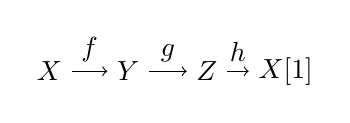
\begin{tikzpicture}[auto,->]
      \node (X) at (0,0) {$X$};
      \node (Y) at (1,0) {$Y$};
      \node (Z) at (2,0) {$Z$};
      \node (X[1]) at (3,0) {$X[1]$};
      \draw (X) -- node {$f$} (Y);
      \draw (Y) -- node {$g$} (Z);
      \draw (Z) -- node {$h$} (X[1]);
    \end{tikzpicture}
  \]
  が与えられているとする.
  次の形で表される図式$\Delta^1 \times \Delta^2 \to \C$
  \[
    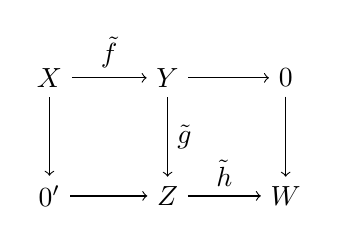
\begin{tikzpicture}[auto,->]
      \node (0') at (0,0) {$0'$};
      \node (Z) at (1.5,0) {$Z$};
      \node (W) at (3,0) {$W$};
      \node (X) at (0,1.5) {$X$};
      \node (Y) at (1.5,1.5) {$Y$};
      \node (0) at (3.0,1.5) {$0$};
      \draw (X) -- node {$\tilde{f}$} (Y);
      \draw (Y) -- node {$\tilde{g}$} (Z);
      \draw (Z) -- node {$\tilde{h}$} (W);
      \draw (Y) -- (0);
      \draw (X) -- (0');
      \draw (0') -- (Z);
      \draw (0) -- (W);
    \end{tikzpicture}
  \]
  が次の条件を満たすとき, $h\C$における上の図式を完全三角(distinguished triangle)という. 
  \begin{enumerate}
    \item 左と右の四角は$\C$のpushoutである. 
    \item $h(\tilde{f}) = f$かつ$h(\tilde{g}) = g$である.
    \item $\tilde{h} : Z \to W$と外の四角により定まる同型$\tilde{i} :W \xrightarrow{\cong} X[1]$の合成に対して, $h = h(\tilde{i} \circ \tilde{h})$である. 
  \end{enumerate}
\end{definition}

\cref{def:distinguished_triangle}の完全三角
\[
  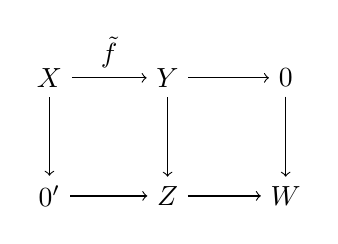
\begin{tikzpicture}[auto,->]
    \node (0') at (0,0) {$0'$};
    \node (Z) at (1.5,0) {$Z$};
    \node (W) at (3,0) {$W$};
    \node (X) at (0,1.5) {$X$};
    \node (Y) at (1.5,1.5) {$Y$};
    \node (0) at (3.0,1.5) {$0$};
    \draw (X) -- node {$\tilde{f}$} (Y);
    \draw (Y) -- (Z);
    \draw (Z) -- (W);
    \draw (Y) -- (0);
    \draw (X) -- (0');
    \draw (0') -- (Z);
    \draw (0) -- (W);
  \end{tikzpicture}
\]
で貼られる$\fun(\Delta^1 \times \Delta^2,\C)$の充満部分圏を$\E$と表す. 

\begin{proposition} \label{prop:homotopy_of_stable_is_triangulated}
  $\C$をコファイバーを持つ基点付き$\infty$圏かつ懸垂$\Sigma : \C \to \C$が圏同値であるとする. 
  このとき, $h\C$, \cref{notation:suspension_and_loop}の懸垂とループ, $\E$の3つ組$(h\C,[-],\E)$は三角圏の構造を持つ.
\end{proposition}

\begin{proof}
  三角圏の公理を順番に示す.
  \begin{description}
    \item[(TR1)] (b) $\E$が同型で閉じていることはpushoutの普遍性などから明らかである.
    (c) 上の図式において$f = \id_X$とすると, $Z$は$0$対象となることから従う.  
    \item[(TR2)] $h\C$における完全三角
    \[
      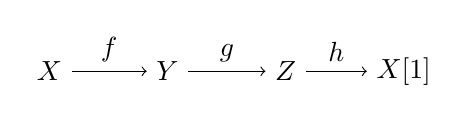
\begin{tikzpicture}[auto,->]
        \node (X) at (0,0) {$X$};
        \node (Y) at (1.5,0) {$Y$};
        \node (Z) at (3,0) {$Z$};
        \node (X[1]) at (4.5,0) {$X[1]$};
        \draw (X) -- node {$f$} (Y);
        \draw (Y) -- node {$g$} (Z);
        \draw (Z) -- node {$h$} (X[1]);
      \end{tikzpicture}
    \]
    を定める$\E$における図式を$\sigma$とする.
    $\sigma$を次の図式に拡張する.
    \[
      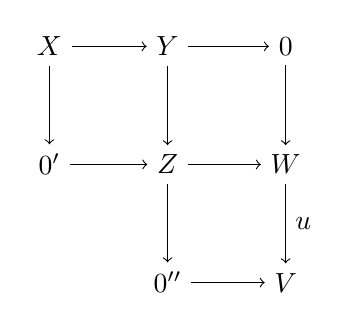
\begin{tikzpicture}[auto,->]
        \node (0') at (0,0) {$0'$};
        \node (Z) at (1.5,0) {$Z$};
        \node (W) at (3,0) {$W$};
        \node (X) at (0,1.5) {$X$};
        \node (Y) at (1.5,1.5) {$Y$};
        \node (0) at (3,1.5) {$0$};
        \node (0'') at (1.5,-1.5) {$0''$};
        \node (V) at (3,-1.5) {$V$};
        \draw (X) -- (Y);
        \draw (Y) -- (Z);
        \draw (Z) -- (W);
        \draw (Y) -- (0);
        \draw (X) -- (0');
        \draw (0') -- (Z);
        \draw (0) -- (W);
        \draw (Z) -- (0'');
        \draw (0'') -- (V);
        \draw (W) -- node {$u$} (V);
      \end{tikzpicture}
    \]
    ここで, 右下の四角はpushoutである.
    次の2つの四角
    \[
      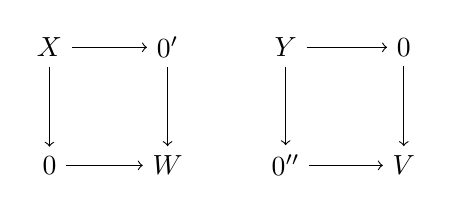
\begin{tikzpicture}[auto,->]
        \node (0') at (0,0) {$0$};
        \node (W) at (1.5,0) {$W$};
        \node (X) at (0,1.5) {$X$};
        \node (0) at (1.5,1.5) {$0'$};
        \node (0'') at (3,0) {$0''$};
        \node (V) at (4.5,0) {$V$};
        \node (Y) at (3,1.5) {$Y$};
        \node (0again) at (4.5,1.5) {$0$};
        \draw (X) -- (0);
        \draw (X) -- (0');
        \draw (0) -- (W);
        \draw (0') -- (W);
        \draw (Y) -- (0again);
        \draw (Y) -- (0'');
        \draw (0again) -- (V);
        \draw (0'') -- (V);
      \end{tikzpicture}
    \]
    の間の射は$h\C$における次の可換図式を定める. 
    \[
      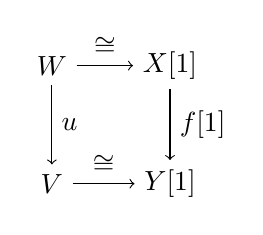
\begin{tikzpicture}[auto,->]
        \node (V) at (0,0) {$V$};
        \node (Y[1]) at (1.5,0) {$Y[1]$};
        \node (W) at (0,1.5) {$W$};
        \node (X[1]) at (1.5,1.5) {$X[1]$};
        \draw (W) -- node {$u$} (V);
        \draw (W) -- node {$\cong$} (X[1]);
        \draw (X[1]) -- node {$f[1]$} (Y[1]);
        \draw (V) -- node {$\cong$} (Y[1]);
      \end{tikzpicture}
    \]
    Lemma.1.1.2.13を右の四角に適応すると, 
    \[
      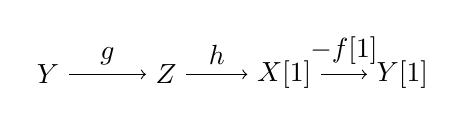
\begin{tikzpicture}[auto,->]
        \node (Y) at (0,0) {$Y$};
        \node (Z) at (1.5,0) {$Z$};
        \node (X[1]) at (3,0) {$X[1]$};
        \node (Y[1]) at (4.5,0) {$Y[1]$};
        \draw (Y) -- node {$g$} (Z);
        \draw (Z) -- node {$h$} (X[1]);
        \draw (X[1]) -- node {$-f[1]$} (Y[1]);
      \end{tikzpicture}
    \]
    は$h\C$における完全三角である. 
    逆に, 次の図式
    \[
      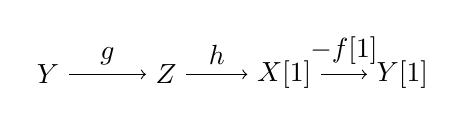
\begin{tikzpicture}[auto,->]
        \node (Y) at (0,0) {$Y$};
        \node (Z) at (1.5,0) {$Z$};
        \node (X[1]) at (3,0) {$X[1]$};
        \node (Y[1]) at (4.5,0) {$Y[1]$};
        \draw (Y) -- node {$g$} (Z);
        \draw (Z) -- node {$h$} (X[1]);
        \draw (X[1]) -- node {$-f[1]$} (Y[1]);
      \end{tikzpicture}
    \]   
    が完全三角であるとする.
    懸垂$\Sigma : \C \to \C$は圏同値なので, 次の図式
    \[
      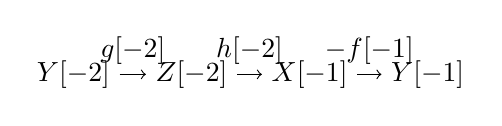
\begin{tikzpicture}[auto,->]
        \node (Y) at (0,0) {$Y[-2]$};
        \node (Z) at (1.5,0) {$Z[-2]$};
        \node (X[1]) at (3,0) {$X[-1]$};
        \node (Y[1]) at (4.5,0) {$Y[-1]$};
        \draw (Y) -- node {$g[-2]$} (Z);
        \draw (Z) -- node {$h[-2]$} (X[1]);
        \draw (X[1]) -- node {$-f[-1]$} (Y[1]);
      \end{tikzpicture}
    \]  
    は完全三角である. 
    先の議論を5回用いると, 次の図式 
    \[
      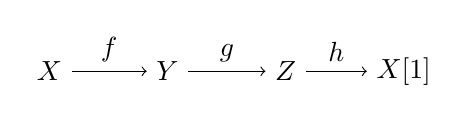
\begin{tikzpicture}[auto,->]
        \node (X) at (0,0) {$X$};
        \node (Y) at (1.5,0) {$Y$};
        \node (Z) at (3,0) {$Z$};
        \node (X[1]) at (4.5,0) {$X[1]$};
        \draw (X) -- node {$f$} (Y);
        \draw (Y) -- node {$g$} (Z);
        \draw (Z) -- node {$h$} (X[1]);
      \end{tikzpicture}
    \]
    は完全三角である. 
    \item[(TR3)] $h\C$における完全三角
    \[
      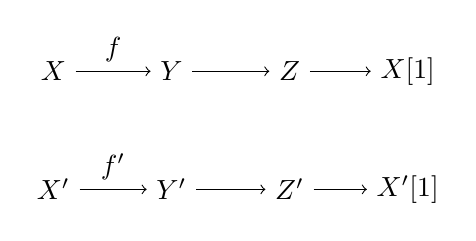
\begin{tikzpicture}[auto,->]
        \node (X') at (0,0) {$X'$};
        \node (Y') at (1.5,0) {$Y'$};
        \node (Z') at (3,0) {$Z'$};
        \node (X'[1]) at (4.5,0) {$X'[1]$};
        \node (X) at (0,1.5) {$X$};
        \node (Y) at (1.5,1.5) {$Y$};
        \node (Z) at (3,1.5) {$Z$};
        \node (X[1]) at (4.5,1.5) {$X[1]$};
        \draw (X') -- node {$f'$} (Y');
        \draw (Y') -- (Z');
        \draw (Z') -- (X'[1]);
        \draw (X) -- node {$f$} (Y);
        \draw (Y) -- (Z);
        \draw (Z) -- (X[1]);
      \end{tikzpicture}
    \]
    を定める$\E$における図式をそれぞれ$\sigma,\sigma'$とする.
    $h\C$における次の可換図式
    \[
      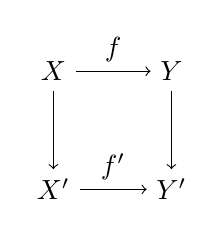
\begin{tikzpicture}[auto,->]
        \node (X') at (0,0) {$X'$};
        \node (Y') at (1.5,0) {$Y'$};
        \node (X) at (0,1.5) {$X$};
        \node (Y) at (1.5,1.5) {$Y$};
        \draw (X) -- node{$f$} (Y);
        \draw (X) -- (X');
        \draw (X') -- node{$f'$} (Y');
        \draw (Y) -- (Y');
      \end{tikzpicture}
    \]
    は$\C$のある四角に(一意とは限らないが)リフトする. 
    この四角を
  \end{description}
\end{proof}

\begin{definition}[Ext群]
  
\end{definition}


\subsection{安定\texorpdfstring{$\infty$}{infty}圏における(余)極限}

安定$\infty$圏の部分圏を定義する. 

\begin{definition}[安定部分圏]
  $\C$を安定$\infty$圏とする.
  $\C_0$を$0$対象を持ち, ファイバーとコファイバーをとる操作で安定であるとする.
  このとき, $\C_0$は安定$\infty$圏であり, $\C_0$を$\C$の安定部分圏(stable subcategory)という. 
\end{definition}

\begin{proof}
  $\C_0$が安定$\infty$圏であることを示す.
  $\C_0$は$0$対象を持つので, (S1)を満たす. 
  $\C_0$はファイバーとコファイバーをとる操作で安定なので, (S2)を満たす. 
  $\C_0$の三角は$\C$の三角なので, $\C$の安定性から, (S3)を満たす. 
\end{proof}

\begin{lemma}
  $\C$を安定$\infty$圏とする.
  $\C_0$をコファイバーとtranslationをとる操作で安定な$\C$の充満部分圏とする.
  このとき, $\C_0$は$\C$の安定部分圏である.
\end{lemma}

\begin{proposition} \label{prop:stable_equiv_limit_and_pullback}
  $\C$を基点付き$\infty$圏とする. 
  $\C$が安定であることと, 次の2つが成立することは同値である. 
  \begin{enumerate}
    \item $\C$は有限極限と有限余極限を持つ. 
    \item $\C$の四角がpushoutであることとpullbackであることは同値である.
  \end{enumerate}
\end{proposition}

\begin{proof}
  (1)と(2)が満たされているとする. 
  (1)は$\C$のファイバーとコファイバーを持つことを示しているので, (S2)を満たす.
  (2)はファイバー列とコファイバー列の同値性を示しているので, (S3)を満たす. 

  逆に, $\C$が安定であるとする. (途中)
\end{proof}

安定$\infty$圏はファイバーとコファイバーのみを用いて定義された. 
しかし, \cref{prop:stable_equiv_limit_and_pullback}より次が従う. 

\begin{corollary} \label{prop:stable_has_limit}
  安定$\infty$圏は有限極限と有限余極限を持つ. 
\end{corollary}

\begin{remark}
  $\C$を安定$\infty$圏とする. 
  \cref{prop:stable_has_limit}より, $\C$は有限極限と有限余極限を持つ. 
  更に, 任意の$X, Y \in \C$に対して, 自然な射
  \begin{align*}
    X \sqcup Y \to X \times Y
  \end{align*}
  が行列
  \begin{align*}
    \begin{pmatrix}
      \id_X & 0 \\
      0 & \id_Y
    \end{pmatrix}
  \end{align*}
  によって与えられる. 
  \cref{prop:homotopy_of_stable_is_triangulated}より, この射は同型である.
  よって, $\C$における$X$と$Y$の直積かつ余直積を$X \otimes Y$と表す. 
\end{remark}

\subsection{完全関手}

基点付き$\infty$圏の間の関手を定義する. 

\begin{definition}[簡約関手]
  $\C,\D$を基点付き$\infty$圏, $\F : \C \to \D$を$\infty$圏の関手とする. 
  $\F$が零対象を保つとき, $\F$は簡約(reduced)であるという.
  簡約関手のなす$\fun(\C,\D)$の部分圏を$\fun_\ast(\C,\D)$と表す. 
\end{definition}

安定$\infty$圏の間の関手を定義する. 

\begin{definition}[完全関手]
  $\C,\D$を安定$\infty$圏, $\F : \C \to \D$を$\infty$圏の関手とする.
  $\F$が$0$対象とファイバー列, コファイバー列を保つとき, $\F$は完全(exact)であるという.
  完全関手のなす$\fun_\ast(\C,\D)$の部分圏を$\fun^\ex(\C,\D)$と表す. 
  また, 安定$\infty$圏と完全関手のなす$\catinf$の部分圏を$\catexinf$と表す. 
\end{definition}

$\F$の完全性は次のように特徴づけることができる. 

\begin{proposition}
  $\F : \C \to \C'$を安定$\infty$圏の関手とする. 
  このとき, 次の3つは同値である. 
  \begin{enumerate}
    \item $\F$は左完全である. つまり, $\F$は有限直積を保つ.
    \item $\F$は右完全である. つまり, $\F$は有限余直積を保つ.
    \item $\F$は完全である.
  \end{enumerate}
\end{proposition}

\begin{proof}
  \cref{prop:Cop_is_also_stable}より, (2)と(3)の同値性を示せばよい. 
  まず, (2)から(3)を示す. 
  $\F$が有限余直積を保つとき, 特に$\F$はコファイバー列を保つ. 
  安定$\infty$圏において, 三角がファイバー列であることとコファイバー列であることは同値であるので, $\F$はファイバー列を保つ. 

  (3)から(2)を示す.
  $\F$が完全であるとする. 
  安定$\infty$圏においてcoequalizerは$\cofib$で表されるので, $\F$はcoequalizerを保つ.
  \cref{prop:hc_is_additive}より, 有限余直積は$\cofib$で表されるので, $\F$は有限余直積を保つ. 
  HTT.4.4.3.2より, $\F$は有限余直積を保つ. 
\end{proof}


\section{安定\texorpdfstring{$\infty$}{infty}圏とHomological Algebra}

\subsection{安定\texorpdfstring{$\infty$}{infty}圏上の\texorpdfstring{$t$}{t}構造}

\begin{definition}[局所化]
  $\C$を$\infty$圏, $\C'$を$\C$の充満部分圏とする. 
  包含$\C' \to \C$が左随伴をもつとき, $\C'$を$\C$の局所化(localization)という. 
\end{definition}

\begin{definition}[安定$\infty$圏上の$t$構造]
  $\C$を安定$\infty$圏とする.
  $h\C$上の$t$構造を$\C$上の$t$構造($t$-structure)という.
  $\C$が$t$構造を持つとき, $(h\C)_{\geq n}$と$(h\C)_{\leq n}$の対象で貼られる$\C$の充満部分圏をそれぞれ$\C_{\geq n}$と$\C_{\leq n}$と表す.
\end{definition}

\begin{proposition} \label{prop:Cleq_is_localization}
  $\C$を$t$構造を持つ安定$\infty$圏とする.
  任意の$n \in \bbZ$に対して, 充満部分圏$\C_{\leq n}$は$\C$の局所化である.
\end{proposition}

\begin{proof}
  $n=-1$のときを示す. 
  HTT.5.2.7.8.より,  任意の$X \in \C$に対して, ある対象$X'' \in \C_{\leq -1}$と射$f : X \to X''$が存在して, 任意の$Y \in \C_{\leq -1}$に対して, 射 
  \begin{align*}
    \Map_\C(X'',Y) \to \Map_\C(X,Y)
  \end{align*}
  が弱ホモトピー同値であることを示せばよい. 
  $t$構造の定義より, ある対象$X' \in \C_{\leq 0}$が存在して, 
  \begin{align*}
    X' \to X \xrightarrow{f} X''
  \end{align*}
  はファイバー列である. 
  Whiteheadの定理より, 任意の$k \leq 0$に対して, 射 
  \begin{align*}
    \Ext_\C^k(X'',Y) \to \Ext_\C^k(X,Y)
  \end{align*}
  がAbel群の同型であることを示せばよい.
  (途中)
\end{proof}

\begin{corollary}
  $\C$を$t$構造を持つ安定$\infty$圏とする.
  $\C$の充満部分圏$\C_{\leq n}$は$\C$における極限で安定である.
  双対的に, $\C$の充満部分圏$\C_{\geq n}$は$\C$における余極限で安定である.
\end{corollary}

\begin{proof}
  $\C_{\leq n}$は$\C$の局所化なので, 包含$\C_{\leq n} \to \C$は右随伴である. 
  よって, $\C_{\leq n}$は$\C$における極限で安定である.
\end{proof}

\begin{definition}[trancation関手]
  $\C$を$t$構造を持つ安定$\infty$圏とする.
  包含$\C_{\leq n} \to \C$の左随伴を$\tau_{\leq n} : \C \to \C_{\leq n}$, 包含$\C_{\geq n} \to \C$の右随伴を$\tau_{\geq n} : \C \to \C_{\geq n}$と表す.
  $\tau_{\leq n}$と$\tau_{\geq n}$をともにtrancation関手(trancation functor)という.
\end{definition}

\begin{remark} \label{rem:trancation_is_on_Cm} 
  $\C$を$t$構造を持つ安定$\infty$圏とする.
  このとき, trancation関手$\tau_{\leq n}, \tau_{\geq n}$は$\C$の充満部分圏$\C_{\leq m}$上の関手である. 
  つまり, 
  \begin{description}
    \item[($m \leq n$)] $\tau_{\leq n} : \C \to \C_{\leq n}$は$\tau_{\leq m}$上の恒等関手に一致する. 
    \item[($m \geq n$)] $\tau_{\leq n} : \C \to \C_{\leq n}$の本質的像は$\C_{\leq m} \subset \C_{\leq n}$に含まれる. 
  \end{description}
\end{remark}

\begin{proof}
  まず, $m \leq n$のときを示す. 
  このとき, $\C_{\leq m} \subset \C_{\leq n}$である. 
  任意の$Y \in \C_{\leq m}$に対して, 
  \begin{align*}
    \Map_{\C_{\leq m}}(\tau_{\leq m}\tau_{\leq n}X,Y)
    \cong \Map_{\C_{\leq n}} (\tau_{\leq n}X,Y) 
    \cong \Map_{\C}(X,Y) 
    \cong \Map_{\C_{\leq m}}(\tau_{\leq m}X,Y)
  \end{align*}
  Yonedaの補題より, $\tau_{\leq m}\tau_{\leq n}X \to \tau_{\leq m}X$は同型である. 
  
  $\tau_{\leq n}\C_{\leq m} = \C_{\leq m}$を示す.
  $\tau_{\leq n}\C_{\leq m} \subset \C_{\leq m}$は上の議論より従う. 
\end{proof}

\begin{corollary}
  $\C$を$t$構造を持つ安定$\infty$圏とする.
  \cref{rem:trancation_is_on_Cm}より, 次の単体的集合の可換図式が存在する.
  \[
    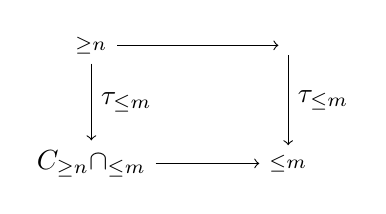
\begin{tikzpicture}[auto,->]
      \node (CnCm) at (0,0) {$C_{\geq n} \cap \C_{\leq m}$};
      \node (Cm) at (2.5,0) {$\C_{\leq m}$};
      \node (Cn) at (0,1.5) {$\C_{\geq n}$};
      \node (C) at (2.5,1.5) {$\C$};
      \draw (Cn) -- (C);
      \draw (Cn) -- node {$\tau_{\leq m}$} (CnCm);
      \draw (C) -- node {$\tau_{\leq m}$} (Cm);
      \draw (CnCm) -- (Cm);
    \end{tikzpicture}
  \]
\end{corollary}

\begin{proof}
  
\end{proof}

\begin{theorem}
  a
\end{theorem}






% \begin{lemma} \label{prop:stable_has_pushout_pullback}
%   $\C$を安定$\infty$圏とする.
%   このとき, 次の2つが成立する.
%   \begin{enumerate}
%     \item $\C$はpushoutとpullbackを持つ. 
%     \item $\C$における四角がpushoutであることとpullbackであることは同値である.
%   \end{enumerate}
% \end{lemma}

% \begin{proof}
%   (1)を示す.
%   \cref{prop:Cop_is_also_stable}より, $\C$がpushoutを持つことを示せばよい.
%   次の図式を考える.
%   \[
%     \begin{tikzpicture}[auto,->]
%       \node (Y) at (0,0) {$Y$};
%       \node (W) at (0,1.5) {$W$};
%       \node (X) at (1.5,1.5) {$X$};
%       \draw (W) -- node {$g$} (X);
%       \draw (W) -- node {$f$} (Y);
%     \end{tikzpicture}
%   \]
%   $f$がファイバーを持つので, 次の図式が存在する.
%   \[
%     \begin{tikzpicture}[auto,->]
%       \node (V) at (-1.5,1.5) {$V$};
%       \node (0) at (-1.5,0) {$0$};
%       \node (Y) at (0,0) {$Y$};
%       \node (W) at (0,1.5) {$W$};
%       \node (X) at (1.5,1.5) {$X$};
%       \draw (V) -- node {$h$} (W);
%       \draw (V) -- (0);
%       \draw (0) -- (Y);
%       \draw (W) -- node {$g$} (X);
%       \draw (W) -- node {$f$} (Y);
%     \end{tikzpicture}
%   \]
%   ここで, 左の四角はファイバー列である.
%   合成$gh$はコファイバーを持ち, 左の四角はコファイバー列でもであるので 次の図式が存在する.
%   \[
%     \begin{tikzpicture}[auto,->]
%       \node (V) at (-1.5,1.5) {$V$};
%       \node (0) at (-1.5,0) {$0$};
%       \node (Y) at (0,0) {$Y$};
%       \node (W) at (0,1.5) {$W$};
%       \node (X) at (1.5,1.5) {$X$};
%       \node (Z) at (1.5,0) {$Z$};
%       \draw (V) -- node {$h$} (W);
%       \draw (V) -- (0);
%       \draw (0) -- (Y);
%       \draw (W) -- node {$g$} (X);
%       \draw (W) -- node {$f$} (Y);
%       \draw (X) -- node {$p$} (Z);
%       \draw (Y) -- (Z);
%     \end{tikzpicture}
%   \]
%   ここで, 外側の四角はpushoutである. 
%   左と外側の四角はpushoutなので, 右側の四角もpushoutである. 

%   (2)を示す.
%   \cref{prop:Cop_is_also_stable}より, 任意のpullbackがpushoutであることを示せばよい.
%   次のpulbackを考える. 
%   \[
%     \begin{tikzpicture}[auto,->]
%       \node (Y) at (0,0) {$Y$};
%       \node (W) at (0,1.5) {$W$};
%       \node (X) at (1.5,1.5) {$X$};
%       \node (Z) at (1.5,0) {$Z$};
%       \draw (W) -- node {$g$} (X);
%       \draw (W) -- node {$f$} (Y);
%       \draw (X) -- node {$p$} (Z);
%       \draw (Y) -- (Z);
%     \end{tikzpicture}
%   \]
%   (1)と同様に, $f$がファイバーを持つので, 次の図式が存在する.
%   \[
%     \begin{tikzpicture}[auto,->]
%       \node (V) at (-1.5,1.5) {$V$};
%       \node (0) at (-1.5,0) {$0$};
%       \node (Y) at (0,0) {$Y$};
%       \node (W) at (0,1.5) {$W$};
%       \node (X) at (1.5,1.5) {$X$};
%       \node (Z) at (1.5,0) {$Z$};
%       \draw (V) -- node {$h$} (W);
%       \draw (V) -- (0);
%       \draw (0) -- (Y);
%       \draw (W) -- node {$g$} (X);
%       \draw (W) -- node {$f$} (Y);
%       \draw (X) -- node {$p$} (Z);
%       \draw (Y) -- (Z);
%     \end{tikzpicture}
%   \]
%   左の四角はファイバー列かつコファイバー列なので, 外側の四角はpullbackかつpushoutである.
%   (1)より, 右の四角はpushoutでもある.
% \end{proof}

% \begin{lemma}
%   $\F : \C \to \D$を安定$\infty$圏の関手とする. 
%   このとき, 次の2つは同値である.
%   \begin{enumerate}
%     \item $\F$は完全である.
%     \item $\F$は零対象とpushoutを保つ.
%     \item $\F$は零対象とpullbackを保つ.
%   \end{enumerate}
% \end{lemma}

% \begin{proof}
%   (2)と(3)の同値性は\cref{prop:stable_has_pushout_pullback}の(2)より従う.\\
%   (1)と(2)の同値性は完全関手がpushoutを保つことを示せばよい. 
%   これは\cref{prop:stable_has_pushout_pullback}の(1)と同様の議論で示せる.
% \end{proof}

% \begin{proposition}
%   $\C$を安定$\infty$圏, $\F : \C \to \D$を安定$\infty$圏の関手とする.
%   このとき, 次の2つが従う. 
%   \begin{enumerate}
%     \item $\C$は任意の有限極限と有限余極限を持つ.
%     \item $\F$が完全であることと, $\F$が有限(余)極限を保つことは同値である. 
%   \end{enumerate}
% \end{proposition}

% \begin{proposition}
%   $\C$を基点付き$\infty$圏とする.
%   このとき, 次の3つは同値である.
%   \begin{enumerate}
%     \item $\C$は安定である.
%     \item $\C$はコファイバーを持ち, 懸垂関手は$\infty$圏同値である. 
%     \item $\C$はファイバーを持ち, ループ関手は$\infty$圏同値である. 
%   \end{enumerate}
% \end{proposition}

% \begin{proof}
%   \cref{prop:Cop_is_also_stable}より, (2)と(3)の同値性は従う. \\
%   (1)から(2)と(1)から(3)はすでに示している.\\
%   (2)から(1)を示す.
%   $\C$をコファイバーを持つ基点付き$\infty$圏, $\Sigma_\C$は$\infty$圏同値であるとする.
%   $\C$が安定であるのは, 次の3つを示せばよい. 
%   \begin{enumerate}
%     \item $\C$の任意のコファイバー列はファイバー列である. 
%     \item $\C$はファイバーを持つ.
%     \item $\C$の任意のファイバー列はコファイバー列である. 
%   \end{enumerate}
% \end{proof}


\end{document}